\section{Markov Chain State Modelling}\label{sec:MCSM}
    Let us suppose that there are two states of market volatility: high (1) and moderate (0).
    We consider the MS-ARIMA (ARIMAX with economy state as an exogenous variable) model for the dynamics of the Nelson-Siegel factors.
    You can see the calibration and forecasting results in \cref{tab:structuralARIMAX,fig:quateryear,fig:yieldraw}



    \begin{figure}[htbp]
        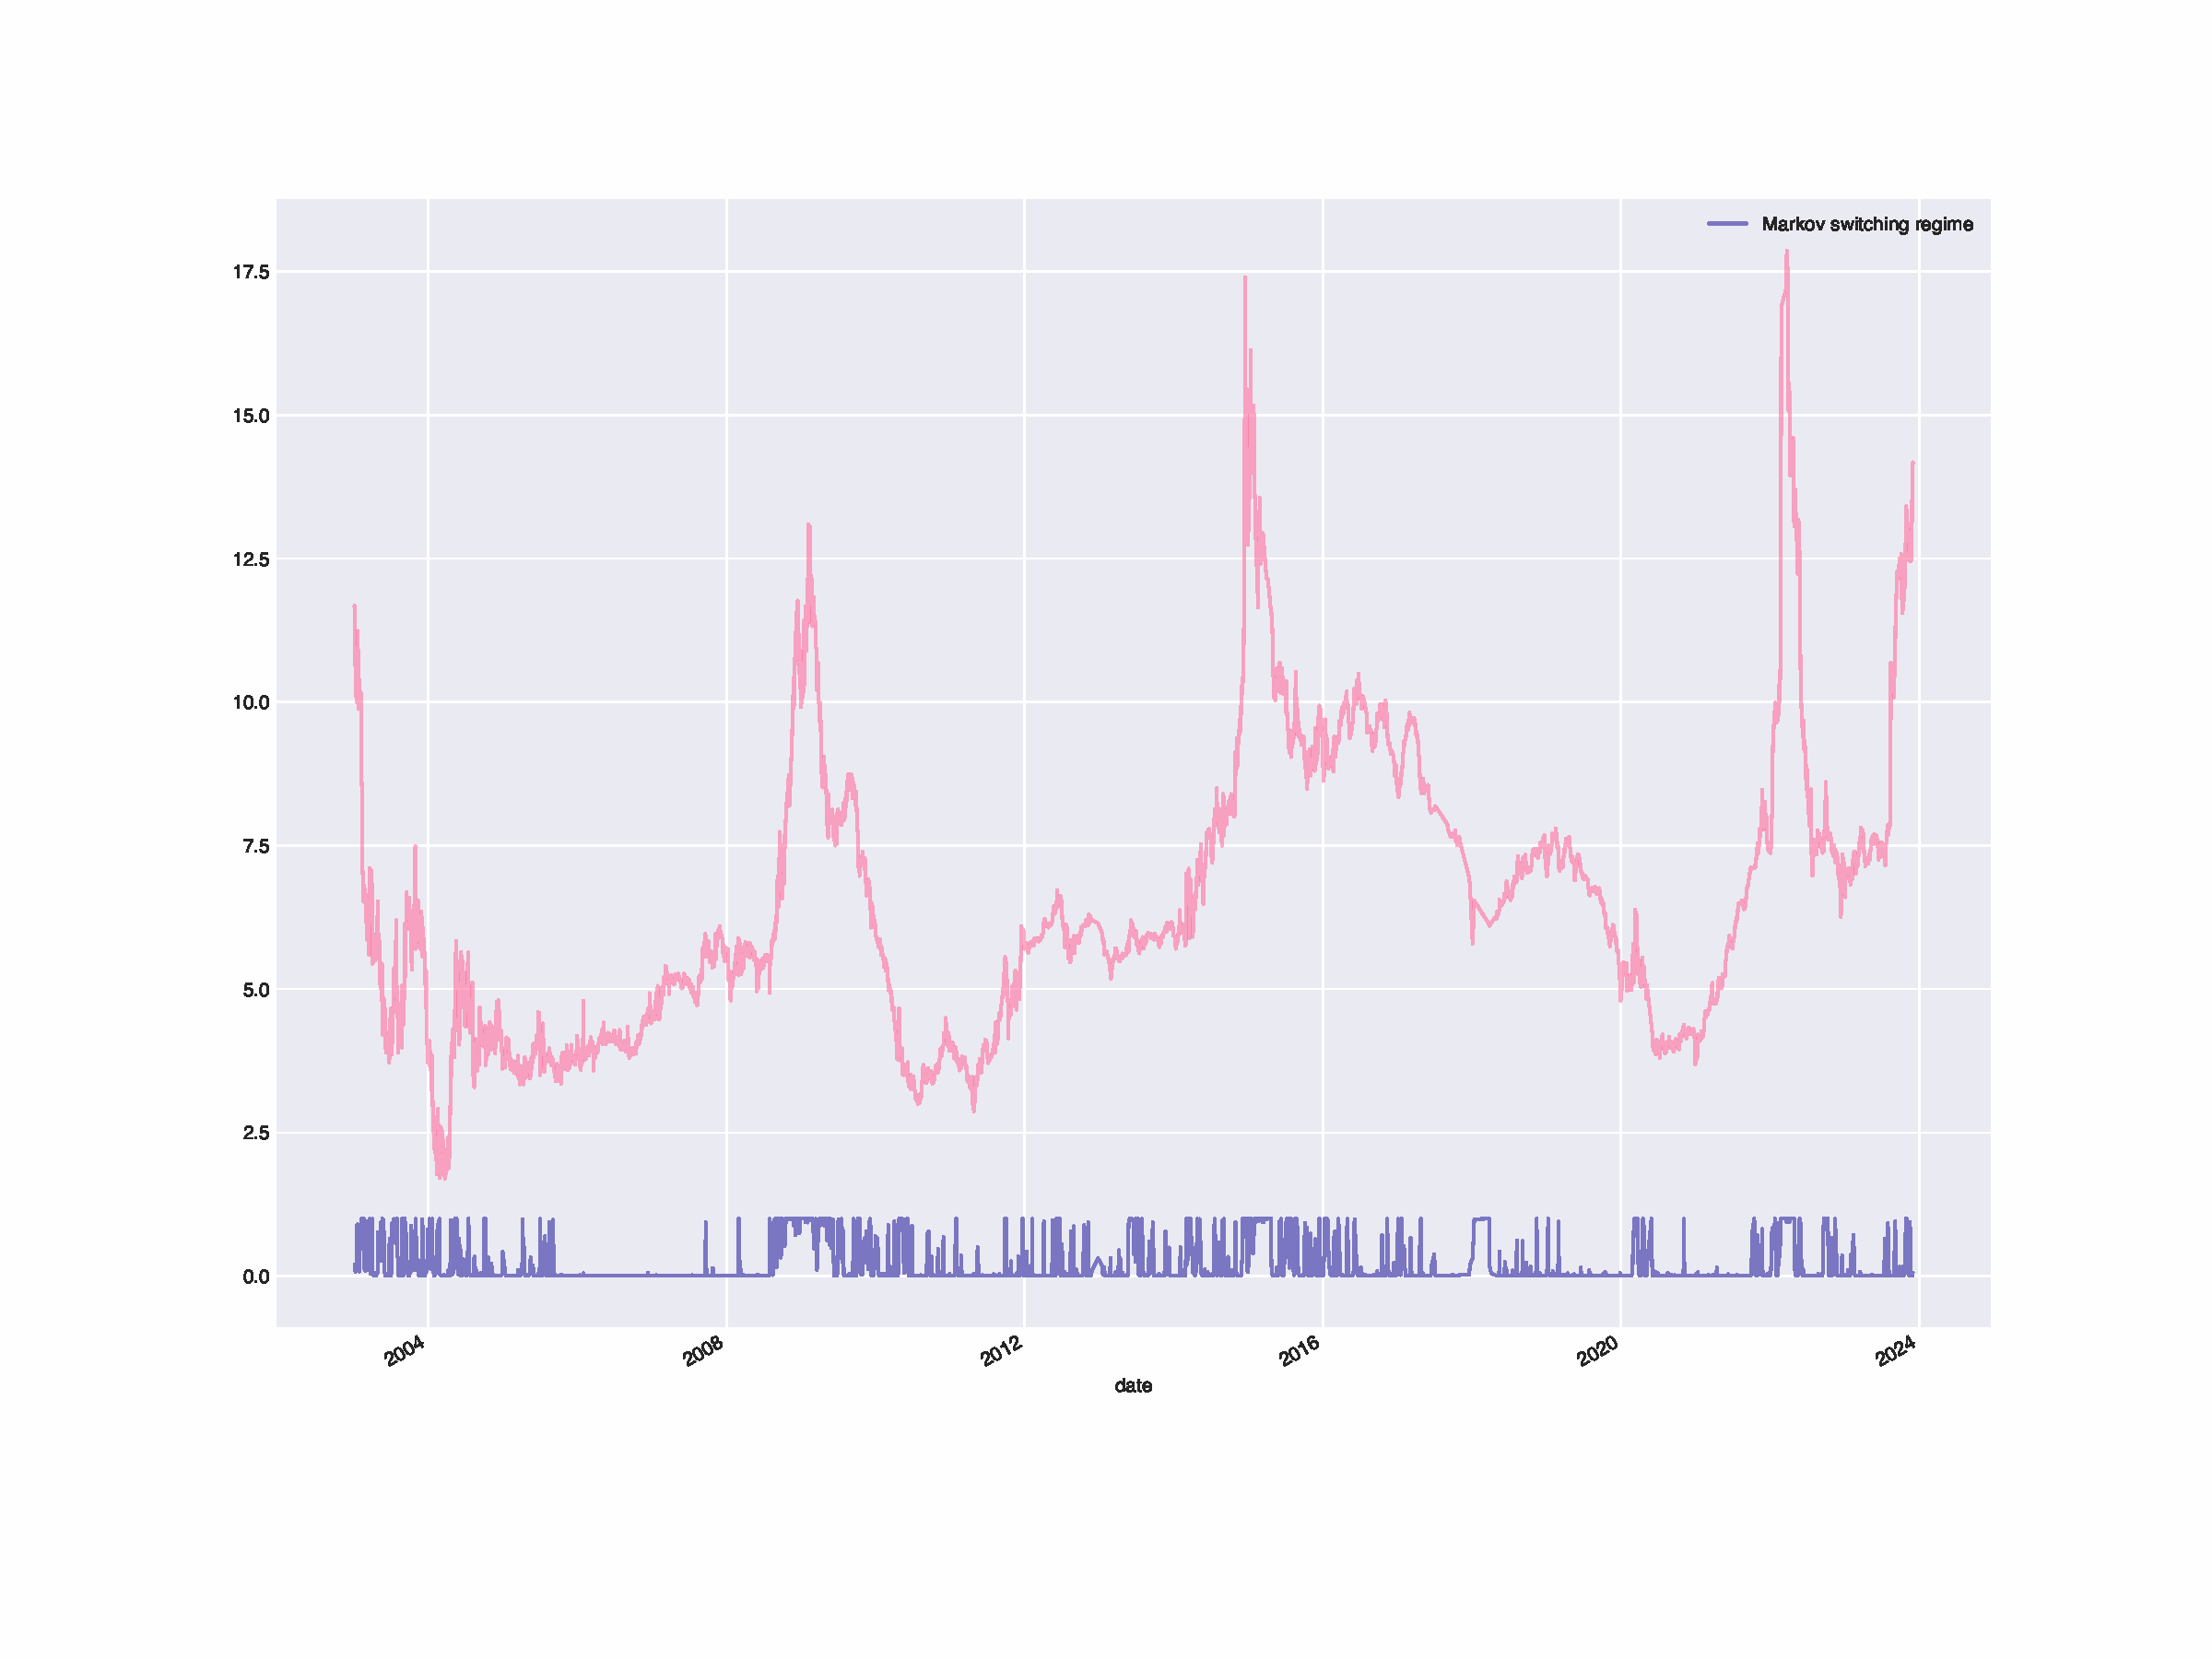
\includegraphics[width=\linewidth]{quateryear_yield_regime.pdf}
        \caption{A bond yield dynamics with 3 moths to maturity.}
        \label{fig:quateryear}
    \end{figure}

    \begin{figure}[htbp]
        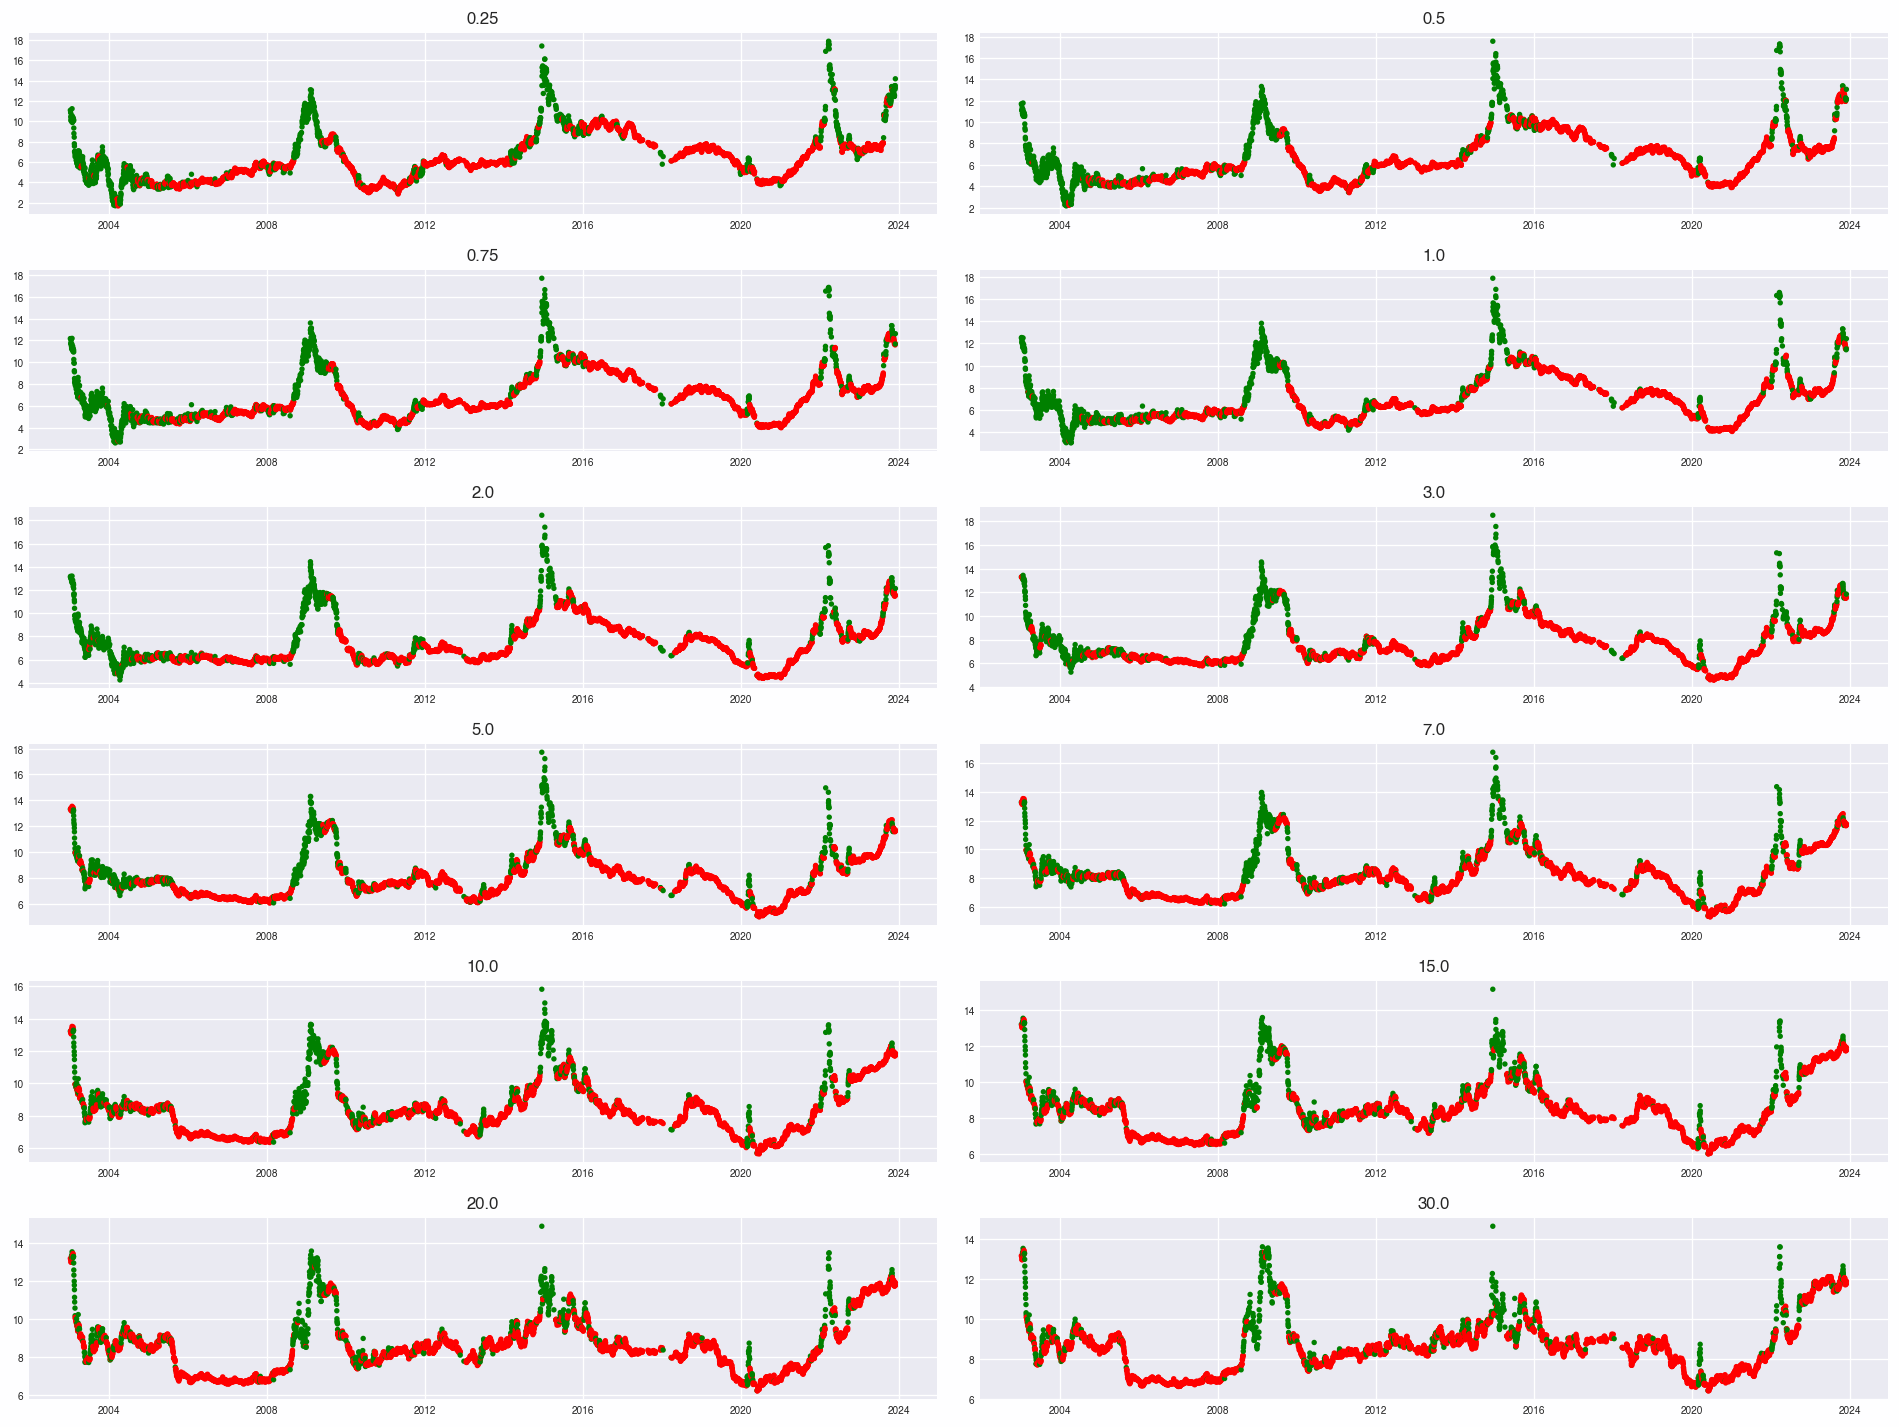
\includegraphics[width=\linewidth]{pointwise_yield_modes.png}
        \caption{Bond-wise yield curve dynamics.}
        \label{fig:yieldraw}
    \end{figure}

    \begin{table}[htbp]
        \centering
        \begin{tabular}{|l|l|l|l|l|l|l|}
        \hline
        Segment            & TTM    & MAPE       & ME       & MAE     & MPE         & RMSE    \\ \hline
        \multirow{4}{*}{0}&0.25&0.009&0.0092&0.0335&0.0026&0.045\\ \cline{2-7}
                        &0.5&0.0084&0.0027&0.0352&0.0008&0.0455\\ \cline{2-7}
                        &0.75&0.0114&-0.0202&0.0523&-0.0043&0.0572\\ \cline{2-7}
                        &1.0&0.0118&-0.0321&0.0583&-0.0064&0.06\\ \cline{2-7}
                        &2.0&0.0123&-0.0695&0.0733&-0.0116&0.0846\\ \cline{2-7}
                        &3.0&0.0094&-0.0609&0.0622&-0.0092&0.078\\ \cline{2-7}
                        &5.0&0.0072&-0.0323&0.0518&-0.0044&0.0596\\ \cline{2-7}
                        &7.0&0.0051&-0.0141&0.0385&-0.0019&0.0438\\ \cline{2-7}
                        &10.0&0.0034&0.0264&0.0264&0.0034&0.0336\\ \cline{2-7}
                        &15.0&0.0053&0.041&0.041&0.0053&0.0475\\ \cline{2-7}
                        &20.0&0.0035&0.0225&0.0279&0.0029&0.0301\\ \cline{2-7}
                        &30.0&0.0017&0.0095&0.0136&0.0012&0.0154\\ \hline
        \multirow{4}{*}{1}&0.25&0.0439&-0.249&0.249&-0.0439&0.2741\\ \cline{2-7}
                        &0.5&0.05&-0.2888&0.2888&-0.05&0.3099\\ \cline{2-7}
                        &0.75&0.0462&-0.272&0.272&-0.0462&0.2952\\ \cline{2-7}
                        &1.0&0.0468&-0.2804&0.2804&-0.0468&0.3003\\ \cline{2-7}
                        &2.0&0.0419&-0.2668&0.2668&-0.0419&0.2852\\ \cline{2-7}
                        &3.0&0.0375&-0.2491&0.2491&-0.0375&0.2676\\ \cline{2-7}
                        &5.0&0.0292&-0.2057&0.2057&-0.0292&0.2463\\ \cline{2-7}
                        &7.0&0.0237&-0.173&0.173&-0.0237&0.2217\\ \cline{2-7}
                        &10.0&0.0179&-0.1346&0.1346&-0.0179&0.2081\\ \cline{2-7}
                        &15.0&0.0149&-0.1149&0.1149&-0.0149&0.1876\\ \cline{2-7}
                        &20.0&0.0137&-0.1073&0.1073&-0.0137&0.1763\\ \cline{2-7}
                        &30.0&0.0065&-0.0338&0.051&-0.0042&0.087\\ \hline
        \multirow{4}{*}{2}&0.25&0.0093&0.0584&0.0584&0.0093&0.0671\\ \cline{2-7}
                        &0.5&0.0067&0.0422&0.0422&0.0067&0.0487\\ \cline{2-7}
                        &0.75&0.0059&0.0374&0.0374&0.0059&0.0463\\ \cline{2-7}
                        &1.0&0.0056&0.0352&0.0352&0.0056&0.0456\\ \cline{2-7}
                        &2.0&0.0057&0.0358&0.0358&0.0057&0.0411\\ \cline{2-7}
                        &3.0&0.0063&0.0398&0.0398&0.0063&0.0423\\ \cline{2-7}
                        &5.0&0.0083&0.0537&0.0537&0.0083&0.0552\\ \cline{2-7}
                        &7.0&0.0112&0.0738&0.0738&0.0112&0.075\\ \cline{2-7}
                        &10.0&0.0151&0.1023&0.1023&0.0151&0.1044\\ \cline{2-7}
                        &15.0&0.0229&0.1611&0.1611&0.0229&0.1703\\ \cline{2-7}
                        &20.0&0.0266&0.1934&0.1934&0.0266&0.2106\\ \cline{2-7}
                        &30.0&0.0276&0.2084&0.2084&0.0276&0.2365\\ \hline
        \multirow{4}{*}{3}&0.25&0.034&0.056&0.3575&0.007&0.4118\\ \cline{2-7}
                        &0.5&0.0312&0.0249&0.3298&0.0039&0.3978\\ \cline{2-7}
                        &0.75&0.0311&0.0488&0.3283&0.006&0.38\\ \cline{2-7}
                        &1.0&0.0312&0.0765&0.3282&0.0086&0.3643\\ \cline{2-7}
                        &2.0&0.0378&0.2548&0.3896&0.0255&0.3924\\ \cline{2-7}
                        &3.0&0.0425&0.3185&0.4347&0.0319&0.4425\\ \cline{2-7}
                        &5.0&0.0471&0.3764&0.4746&0.0381&0.49\\ \cline{2-7}
                        &7.0&0.0467&0.3558&0.4641&0.0366&0.4766\\ \cline{2-7}
                        &10.0&0.0419&0.2572&0.4115&0.0272&0.4154\\ \cline{2-7}
                        &15.0&0.0338&0.1591&0.3281&0.0173&0.3337\\ \cline{2-7}
                        &20.0&0.0272&0.0828&0.2627&0.0094&0.2815\\ \cline{2-7}
                        &30.0&0.0207&0.0099&0.2&0.0017&0.2481\\ \hline

        \end{tabular}
        \caption{MS-ARIMA forecasting results for the structural NS factors.}
        \label{tab:structuralARIMAX}
    \end{table}

